\documentclass[a4paper,11pt]{article}
\usepackage[utf8]{inputenc}
\usepackage[T1]{fontenc}
\usepackage[swedish]{babel}
\usepackage{amsmath,amssymb,amsfonts}
\usepackage{graphicx}
\usepackage{enumitem}
\usepackage{geometry}
\usepackage{tikz}
\geometry{margin=2.5cm}

\title{Repetitionsuppgifter -- Matematik 1}
\author{}
\date{\today}

\begin{document}

\maketitle

\section*{Grundläggande ekvationslösning och olikheter}

\begin{enumerate}[label=\textbf{\arabic*.}]
    \item Lös ekvationen: $2x + 3 = 7$
    
    \item Lös ekvationen: $3x - 5 = 10$
    
    \item Lös ekvationen: $5x + 2 = 3x - 4$
    
    \item Lös ekvationen: $\frac{x}{3} + 2 = 5$
    
    \item Lös ekvationen: $2(x + 3) = 4x - 6$
    
    \item Lös ekvationen: $\frac{x+1}{2} = \frac{x-3}{4}$
    
    \item Lös ekvationen: $3(x - 1) - 2(x + 3) = 5$
    
    \item Lös ekvationen: $\frac{2x-1}{3} + \frac{x+2}{4} = 2$
    
    \item Lös olikheten: $2x + 3 < 7$
    
    \item Lös olikheten: $3x - 5 \geq 10$
    
    \item Lös olikheten: $5x + 2 > 3x - 4$
    
    \item Lös olikheten: $\frac{x}{3} + 2 \leq 5$
    
    \item Lös olikheten: $2(x + 3) < 4x - 6$
    
    \item Lös olikheten: $-3 < 2x - 5 < 7$
    
    \item Lös olikheten: $\frac{x-1}{2} > \frac{x+3}{4}$
    
    \item Lös olikheten: $3(x - 1) - 2(x + 3) \leq 5$
\end{enumerate}

\newpage
\section{Räta linjens ekvation}
\begin{enumerate}[label=\textbf{\arabic*.}]
    \item Vad är lutningen för linjen $y = 2x + 1$?
    \item Vad är $y$-värdet när $x = 0$ för linjen $y = -3x + 4$?
    \item Bestäm räta linjens ekvation som går genom punkten $(0,2)$ och har lutningen $k=3$.
    \item Bestäm räta linjens ekvation som går genom punkterna $(1,2)$ och $(3,6)$.
    \item För linjen $y = -x + 5$, bestäm $x$ när $y = 0$.
    \item Bestäm räta linjens ekvation som går genom punkterna $(-2,2)$ och $(4,-10)$.
    \item \textbf{Grafanalys:} Nedan visas grafen till en linje. Svara på frågorna.
    \begin{center}
    \begin{tikzpicture}[scale=0.8]
  % Axlar
  \draw[->] (-1,0) -- (5,0) node[right] {$x$};
  \draw[->] (0,-1) -- (0,5) node[above] {$y$};
  % x-ticks
  \foreach \x in {0,1,2,3,4}
    \draw (\x,0.1) -- (\x,-0.1) node[below] {$\x$};
  % y-ticks
  \foreach \y in {0,1,2,3,4}
    \draw (0.1,\y) -- (-0.1,\y) node[left] {$\y$};
  % Linje
  \draw[thick,blue] (-2,-1) -- (4,5);
\end{tikzpicture}
    \end{center}
    a) Vad är linjens lutning?
    
    b) Vad är linjens ekvation?
    
    c) Var skär linjen $y$-axeln?
\end{enumerate}
\newpage
% Linjära funktioner
\section{Linjära funktioner}
\begin{enumerate}[label=\textbf{\arabic*.}]
    \item För funktionen $f(x) = 2x + 3$, beräkna $f(0)$, $f(2)$ och $f(-1)$.
    \item För funktionen $g(x) = -x + 4$, bestäm $x$ då $g(x) = 1$.
    \item För vilka $x$ gäller $f(x) = g(x)$ om $f(x) = 2x + 3$ och $g(x) = -x + 4$?
    \item \textbf{Grafanalys:} Nedan visas grafen till funktionen $h(x) = -0.5x + 2$.
    \begin{center}
    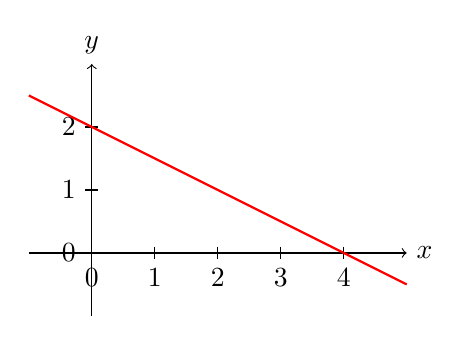
\begin{tikzpicture}[scale=0.8]
  % Axlar
  \draw[->] (-1,0) -- (5,0) node[right] {$x$};
  \draw[->] (0,-1) -- (0,3) node[above] {$y$};
  % x-ticks
  \foreach \x in {0,1,2,3,4}
    \draw (\x,0.1) -- (\x,-0.1) node[below] {$\x$};
  % y-ticks
  \foreach \y in {0,1,2}
    \draw (0.1,\y) -- (-0.1,\y) node[left] {$\y$};
  % Linje
  \draw[thick,red] (-1,2.5) -- (5,-0.5);
\end{tikzpicture}
    \end{center}
    a) Vad är nollstället för $h(x)$?
    
    b) Vad är $h(2)$?
\end{enumerate}
\newpage
% Exponentialfunktioner
\section{Exponentialfunktioner}
\begin{enumerate}[label=\textbf{\arabic*.}]
    \item För funktionen $f(x) = 2^x$, beräkna $f(0)$, $f(1)$, $f(2)$.
    \item För funktionen $g(x) = 3 \cdot 2^x$, bestäm $g(0)$ och $g(2)$.
    \item En exponentialfunktion $h(x) = a \cdot b^x$ har värdet $h(0) = 5$ och $h(1) = 10$. Bestäm $a$ och $b$.
    \item \textbf{Grafanalys:} Nedan visas grafen till funktionen $p(x) = 2^x$.
    \begin{center}
    \begin{tikzpicture}[scale=0.8]
  % Axlar
  \draw[->] (-1,0) -- (4,0) node[right] {$x$};
  \draw[->] (0,-1) -- (0,9) node[above] {$y$};
  % x-ticks
  \foreach \x in {0,1,2,3}
    \draw (\x,0.2) -- (\x,-0.2) node[below] {$\x$};
  % y-ticks
  \foreach \y in {0,2,4,6,8}
    \draw (0.2,\y) -- (-0.2,\y) node[left] {$\y$};
  % Graf
  \draw[thick,green!70!black,domain=-1:3,samples=40] plot (\x,{2^\x});
\end{tikzpicture}
    \end{center}
    a) Vilket värde har $p(2)$?
    
    b) Vad är $p(0)$?
    
    c) Hur förändras $p(x)$ när $x$ ökar med 1?
\end{enumerate}
\newpage
% Problemlösning med funktioner
\section{Problemlösning med funktioner}
\begin{enumerate}[label=\textbf{\arabic*.}]
    \item En biobiljett kostar 90 kr. Skriv en funktion $C(x)$ som beskriver totalkostnaden för $x$ biljetter. Vad kostar 5 biljetter?
    \item En cykelbutik hyr ut cyklar för 80 kr per dag plus en fast avgift på 50 kr. Skriv en funktion $H(x)$ för hyran av $x$ dagar. Vad kostar det att hyra i 3 dagar?
    \item En bakteriekultur fördubblas varje timme och startar med 10 bakterier. Skriv en funktion $N(t)$ som beskriver antalet bakterier efter $t$ timmar. Hur många bakterier finns efter 4 timmar?
    \item Nedan visas grafen till en funktion $f(x)$ av tredje graden.
    \begin{center}
    \begin{tikzpicture}[scale=0.8]
      % Axlar
      \draw[->] (-3,0) -- (4,0) node[right] {$x$};
      \draw[->] (0,-3) -- (0,5) node[above] {$y$};
      % x-ticks
      \foreach \x in {-2,-1,1,2,3}
        \draw (\x,0.15) -- (\x,-0.15) node[below] {$\x$};
      % y-ticks
      \foreach \y in {-2,2,4}
        \draw (0.15,\y) -- (-0.15,\y) node[left] {$\y$};
      % Graf: t.ex. f(x) = (x+2)(x-1)(x-3)/2 + 1
      \draw[thick,blue,domain=-2.2:3.2,samples=100,smooth] plot (\x,{((\x+2)*(\x-1)*(\x-3))/2 + 1});
    \end{tikzpicture}
    \end{center}
    a) Vad är $f(0)$?
    
    b) För vilka $x$ gäller $f(x) = 0$?

    \item Nedan visas grafen till en annan funktion $g(x)$ av tredje graden.
    \begin{center}
    \begin{tikzpicture}[scale=0.8]
      % Axlar
      \draw[->] (-4,0) -- (4,0) node[right] {$x$};
      \draw[->] (0,-4) -- (0,4) node[above] {$y$};
      % x-ticks
      \foreach \x in {-3,-2,-1,1,2,3}
        \draw (\x,0.15) -- (\x,-0.15) node[below] {$\x$};
      % y-ticks
      \foreach \y in {-2,2}
        \draw (0.15,\y) -- (-0.15,\y) node[left] {$\y$};
      % Graf: t.ex. g(x) = (x+3)(x)(x-2)/3
      \draw[thick,red,domain=-3.3:2.3,samples=100,smooth] plot (\x,{((\x+3)*(\x)*(\x-2))/3});
    \end{tikzpicture}
    \end{center}
    a) Vad är $g(0)$?
    
    b) För vilka $x$ gäller $g(x) = 0$?

\end{enumerate}






\newpage
\section*{Procent och förändringsfaktor}

\begin{enumerate}[label=\textbf{\arabic*.}]
    \item Beräkna:
    \begin{enumerate}[label=\alph*)]
        \item 15\% av 400
        \item 7,5\% av 80
        \item 120\% av 50
    \end{enumerate}
    
    \item Hur många procent är:
    \begin{enumerate}[label=\alph*)]
        \item 30 av 150
        \item 45 av 180
        \item 5 av 25
    \end{enumerate}
    
    \item Ett klädesplagg kostar 800 kr. Under en rea sänks priset med 25\%.
    \begin{enumerate}[label=\alph*)]
        \item Vad blir det nya priset?
        \item Vilken förändringsfaktor motsvarar prissänkningen?
    \end{enumerate}
    
    \item En vara kostar 500 kr. Priset höjs med 12\%.
    \begin{enumerate}[label=\alph*)]
        \item Vad blir det nya priset?
        \item Vilken förändringsfaktor motsvarar prishöjningen?
    \end{enumerate}
    
    \item Priset på en vara höjs från 200 kr till 250 kr.
    \begin{enumerate}[label=\alph*)]
        \item Hur många procent höjs priset?
        \item Vilken förändringsfaktor motsvarar prishöjningen?
    \end{enumerate}
    
    \item Antalet invånare i en stad minskar från 45 000 till 40 500.
    \begin{enumerate}[label=\alph*)]
        \item Hur många procent minskar befolkningen?
        \item Vilken förändringsfaktor motsvarar minskningen?
    \end{enumerate}
    
    \item En vara kostar 400 kr. Priset höjs först med 20\% och sedan med ytterligare 10\%.
    \begin{enumerate}[label=\alph*)]
        \item Vad blir det slutliga priset?
        \item Hur många procent har priset totalt höjts med?
        \item Vilken förändringsfaktor motsvarar den totala prishöjningen?
    \end{enumerate}
    
    \item En vara kostar 600 kr. Under en rea sänks priset med 30\%. Efter rean höjs priset med 40\%.
    \begin{enumerate}[label=\alph*)]
        \item Vad blir det slutliga priset?
        \item Hur många procent har priset totalt förändrats med?
        \item Vilken förändringsfaktor motsvarar den totala prisförändringen?
    \end{enumerate}
\end{enumerate}


\newpage
\section*{Sannolikhet}

\subsection*{Enkla slumpförsök}

\begin{enumerate}[label=\textbf{\arabic*.}]
    \item En vanlig tärning kastas en gång. Beräkna sannolikheten för att:
    \begin{enumerate}[label=\alph*)]
        \item Få en 6:a
        \item Få ett jämnt tal
        \item Få ett tal som är större än 4
    \end{enumerate}
    
    \item En kortlek med 52 kort innehåller 13 kort av varje färg (hjärter, ruter, klöver, spader). Beräkna sannolikheten för att dra:
    \begin{enumerate}[label=\alph*)]
        \item Ett hjärter
        \item Ett ess (det finns ett ess i varje färg)
        \item Ett svart kort (klöver och spader är svarta)
    \end{enumerate}
    
    \item I en urna finns 5 röda, 3 blå och 2 gröna kulor. En kula dras slumpmässigt. Beräkna sannolikheten för att:
    \begin{enumerate}[label=\alph*)]
        \item Kulan är röd
        \item Kulan är blå eller grön
        \item Kulan är varken röd eller blå
    \end{enumerate}
    
    \item I en klass med 30 elever är 18 flickor och 12 pojkar. Av flickorna har 6 glasögon och av pojkarna har 4 glasögon. En elev väljs slumpmässigt. Beräkna sannolikheten för att:
    \begin{enumerate}[label=\alph*)]
        \item Eleven är en flicka
        \item Eleven har glasögon
        \item Eleven är en pojke med glasögon
    \end{enumerate}
\end{enumerate}

\subsection*{Slumpförsök i flera steg}

\begin{enumerate}[label=\textbf{\arabic*.}]
    \item En vanlig tärning kastas två gånger. Beräkna sannolikheten för att:
    \begin{enumerate}[label=\alph*)]
        \item Få två 6:or
        \item Få summan 7
        \item Få minst en 6:a
    \end{enumerate}
    
    \item Två vanliga tärningar kastas samtidigt. Beräkna sannolikheten för att:
    \begin{enumerate}[label=\alph*)]
        \item Få samma tal på båda tärningarna
        \item Få summan 8
        \item Få en summa som är högst 4
    \end{enumerate}
    
    \item Från en kortlek med 52 kort dras två kort i följd utan återläggning. Beräkna sannolikheten för att:
    \begin{enumerate}[label=\alph*)]
        \item Båda korten är ess
        \item Första kortet är ett ess och andra kortet är en kung
        \item Båda korten är röda (hjärter och ruter är röda)
    \end{enumerate}
    \break
    \item I en urna finns 4 vita och 6 svarta kulor. Två kulor dras slumpmässigt utan återläggning. Beräkna sannolikheten för att:
    \begin{enumerate}[label=\alph*)]
        \item Båda kulorna är vita
        \item Båda kulorna är svarta
        \item En kula är vit och en kula är svart
    \end{enumerate}
    
    \item En påse innehåller 3 röda, 2 blå och 1 grön kula. Du drar slumpmässigt två kulor i följd utan återläggning.
    \begin{enumerate}[label=\alph*)]
        \item Rita ett träddiagram för detta slumpförsök.
        \item Beräkna med hjälp av träddiagrammet sannolikheten att få två kulor med olika färg.
        \item Beräkna sannolikheten att få minst en röd kula.
    \end{enumerate}
    
    \item En skola har två klasser med 20 elever i varje klass. I klass A är 12 elever flickor och i klass B är 8 elever flickor. En elev väljs slumpmässigt från hela skolan genom att först välja en klass och sedan en elev från den valda klassen.
    \begin{enumerate}[label=\alph*)]
        \item Rita ett träddiagram för detta slumpförsök.
        \item Beräkna med hjälp av träddiagrammet sannolikheten att den valda eleven är en flicka.
        \item Om den valda eleven visar sig vara en flicka, vad är sannolikheten att hon kommer från klass A?
    \end{enumerate}
\end{enumerate}

\end{document}
